\chapter{An Investigation in Using DDSP to Learn and Synthesize Vocal Features}

The adaptation of DDSP to synthesize vocal features such as singing using the additional MFFC layer was chosen for further investigation.

All research was undertaken using Google Colab notebooks and cloud hardware, primarily NVIDIA Tesla V100 GPUs.

Two seperate models were trained, one for a male voice (Chris Martin from Coldplay) and one for a female voice (Taylor Swift). This was done to see how the DDSP architecture would handle different vocies e.g. Alto or Tennor differently.

It was hypothesized that 2 albums would be the optimal size for any training dataset. Premilinary investigations on smaller datasets yielded significant overfitting and poor performance when any of the F0, amplitude latent features were modified during inference. Datasets of any greater size would be preferred. However, larger models would be slower to train.

\begin{figure}
    \centering
    \caption{Songs and albums going into each training dataset}
\end{figure}

\section{Dataset Preparation}

\subsection{Source Separation}

Following the selection of the two albums for each artist and removal of any songs where additional vocal artists to the main vocalist featured were removed, all songs were passed through the pre-trained Spleeter model\cite{SpleeterPip}\cite{SpleeterPip}. This pre-trained model can carry out source separation of instrumental and music tracks. Source separation was essential as the training dataset must not contain any instrumentals. The model outputted two separate tracks for each song, one representing the instrumentals and one the vocals. The instrumental tracks were discarded.

Using Spleeter to split existing songs with instrumental components opened up the possibility of using a more significant number of songs, something the original singing DDPS paper's authors did not consider. Their largest single voice dataset had a compressed size of ~70Mb, whereas the pre-processed datasets used in this paper were approximately ten times that at ~700Mb, whilst still being based on a single vocal artist, style of music, and vocals only tracks. Using a more extensive training dataset would reduce over-fitting and aid generalisation.

The remaining vocal tracks were then pre-processed.

\subsection{Pre-processing}

\begin{figure}[H]
    \centering
    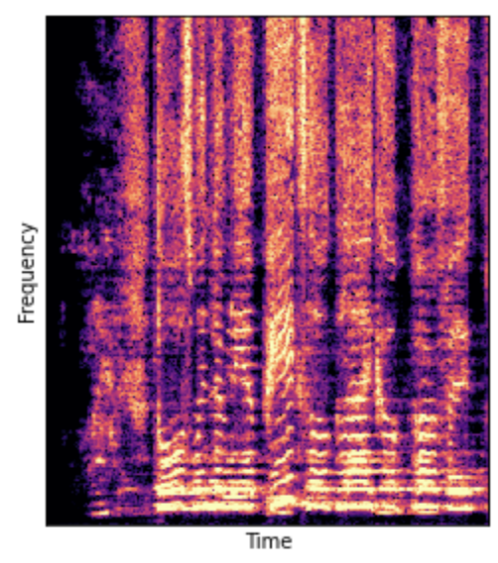
\includegraphics[width=0.6\textwidth]{research/dataset_preparation/PreprocessingSpecplot.png}
    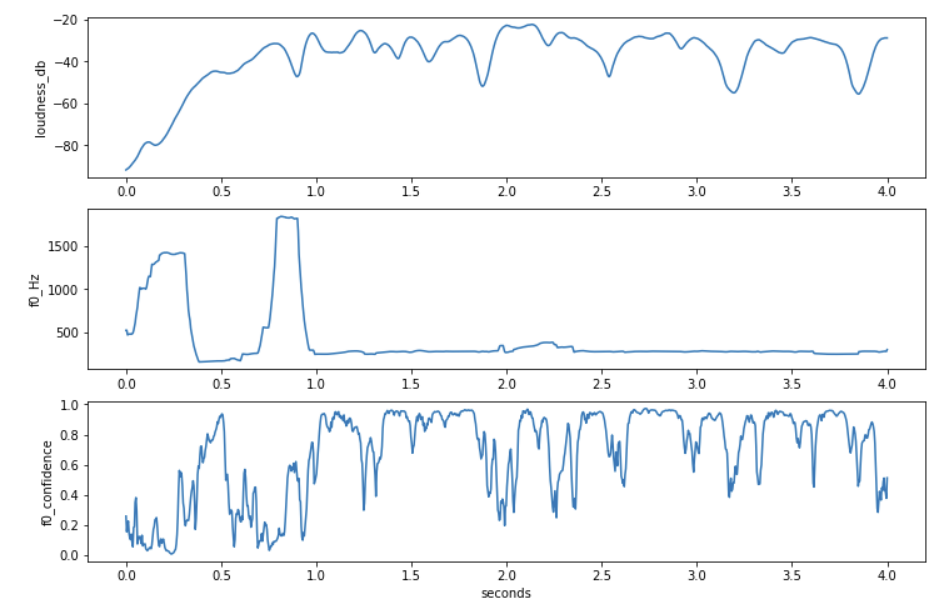
\includegraphics[width=0.8\textwidth]{research/dataset_preparation/PreprocessingFeatures.png}
    \caption{Dataset Pre-processing: Spectrogram plot of a random 4 second sample from one of the datasets and its accomanying F0, F0 Confidence and Amplitude characteristics over time throughout the sample}
\end{figure}

Pre-processing the datasets involved splitting the raw audio into smaller frames (samples), each 4 seconds long. The frame length was limited to 4 seconds to avoid capturing too much information in one spectrogram, which would make learning using the convolutional neural network difficult.

For each frame, F0 and confidence of F0 probability were inferred using CREPE\cite{CREPE}. Amplitude was computed statistically using the Librosa library\cite{LibrosaPip}. Latent Z information was available through the passing of the raw audio. The 4-second samples and accompanying features were then stored as TFRecord files.

Each of the two datasets was pre-processed on Google Colab notebooks; this process took approximately 40 minutes for each dataset using an NVIDIA Tesla V100 GPU.

Finally, a random 4-second clip was selected from each dataset to prove successful pre-processing. Its spectrogram was computed and plotted. Computed F0, F0 Confidence and Amplitude characteristics were also plotted for the selected clip. The underlying audio sample could also be played.

\section{Training}

A preprocessor was used that resampled the fundamental frequency and loudness, taking account the sample rate, frame rate, and number of timesteps. The number of timesteps was set at 1000 per 4 second clip, giving a spectral resoluiton of 4ms per timestep. This was deemed to be the best compromise between computational efficiency and accuracy.

An autoencoder encoder decoder setup was used. The encoder was based on Mfcc variant of a \acrfull{RNN}. The decoder was a RNN based decoder as described previously in \nameref{sec:singing_voice_synthesis}.

The model settings were kept the same as in \nameref{sec:singing_voice_synthesis} as they had already validated their hyperparameter selection. This included the use of100 sinusoidal harmonic components and 60 filter banks. This was done to limit model size to ensure it fitted on one GPU.

Each model was trained for 200,000 epochs, training time was approximately 2.9 epochs per second or 5.2 epochs per second depending on GPU used. Total training time was approxumately 20 horus per model.

\begin{figure}[!ht]
    \centering
    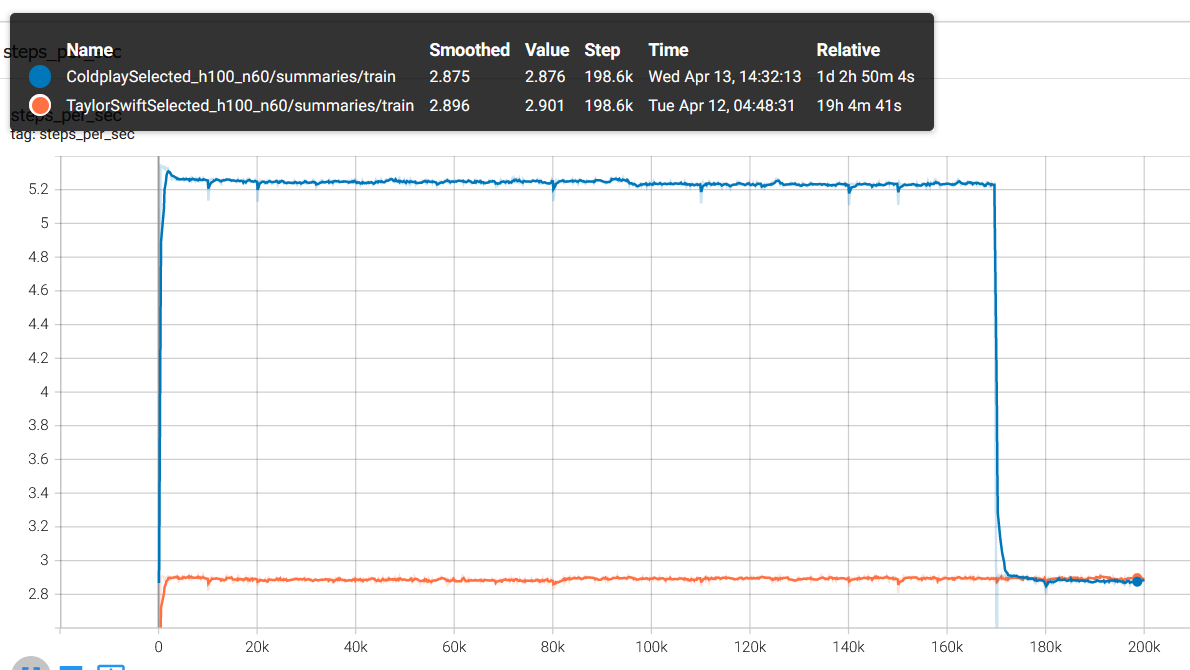
\includegraphics[width=0.6\textwidth]{research/training/StepsPerSecond.png}
    \caption{Training steps per second over the 200,000 training epochs}
\end{figure}

\begin{figure}[!ht]
    \centering
    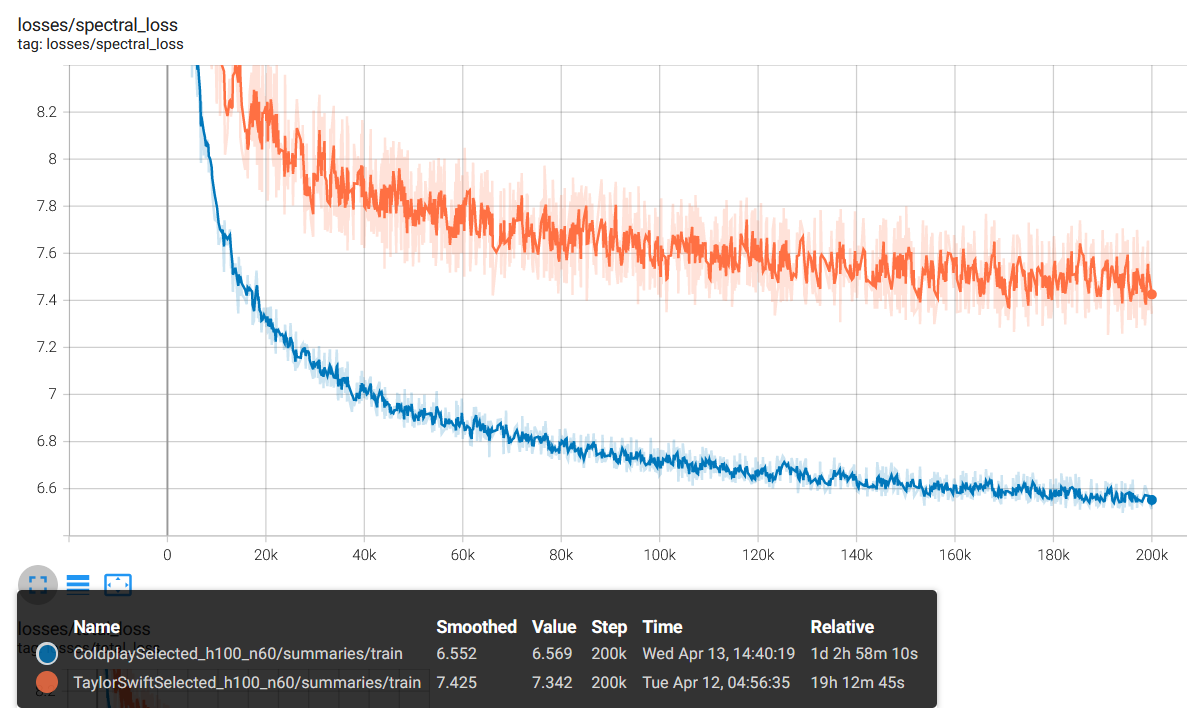
\includegraphics[width=0.8\textwidth]{research/training/TrainingSpectralLosses.png}
    \caption{Training Spectral Losses: Losses over the 200,000 epochs of training both models, using the spectral loss function defined in \nameref{sec:loss_measure}}
    \label{fig:training_spectral_losses}
\end{figure}

\nameref{fig:training_spectral_losses} shows the Coldplay losses being less than the Taylor Swift losses. This is due to the fact that the Coldplay Dataset having more frames that were pure silence, meaning that the Coldplay model fitted the silence frames more accurately.



\section{Results}

Several inferencing tests were conducted to see if the models had learned the latent features correctly to evaluate the models' performance.

All inferencing tests took approximately 0.3 seconds for a 4-minute frame; this is fast enough to enable real-time applications and significantly quicker than the Jukebox model.

\subsection{Recreation from the Training Dataset}

A random frame was selected and passed through each model; loudness and F0 were unmodified. The results of the inferencing were then compared to the original training dataset.

Each model successfully recreated original frames, though the Taylor Swift dataset yielded the best results.

Timbral features were slightly distorted (more so with the Coldplay model), but the overall quality was good, and it was easy to tell it was the original singer in both cases. In addition, pitch estimation was highly accurate and in line with the original pitch. Pitch accuracy can be partially attributed to the accuracy of the CREPE pitch detection model\cite{CREPE} and because the pitch was directly passed to the harmonic synthesiser.

The resynthesis of understandable words from the original frame was a far more considerable achievement. The original singing DDSP paper\cite{SingingDDSP} suffered a problem of stuttering when attempting resynthesis as their model was unable to recreate phonemes of the human voice accurately. It is possible that using far larger datasets has improved the quality of the resynthesis because the models had become more general in their ability to synthesise the human voice. However, it must be said that the Coldplay model was harder to understand.

\begin{figure}[H]
    \centering
    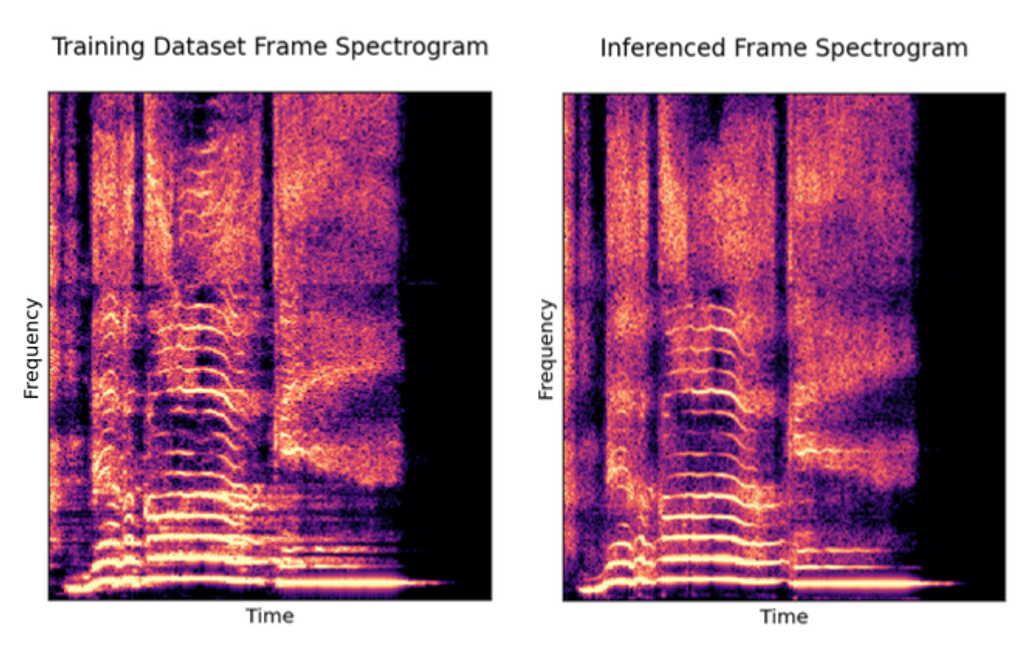
\includegraphics[width=0.8\textwidth]{research/results/TaylorSwift/InferredRecreation.png}
    \caption{(Taylor Swift) Original and resynthesized frames without latent modification}
\end{figure}

\begin{figure}[H]
    \centering
    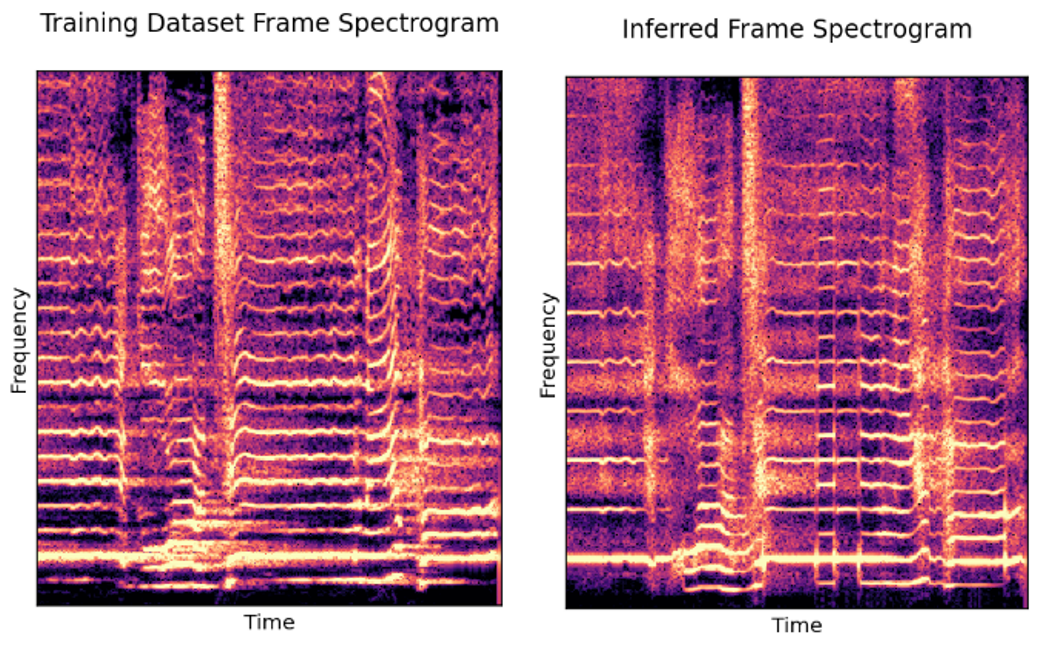
\includegraphics[width=0.8\textwidth]{research/results/Coldplay/InferredRecreation.png}
    \caption{(Coldplay) Original and resynthesized frames without latent modification}
\end{figure}

\subsection{F0 Pitch Transposition by a fixed octave}

A more advanced inferencing test was then undertaken. The fundamental frequency latent as determined by CREPE was transposed by fixed octaves (-2, -1, 0, 0.5, 1, 2), and the inferencing was re-performed on the transposed latents. Both models responded to the change in F0 and could accurately transpose harmonic pitch by the correct octave amount. At minor transpositions, e.g. +1 or -1 octave, the inferred frame still sounded somewhat like a human voice. However, it sounded like the noise, and harmonic components were separate sources at greater transpositions and did not constitute one voice.

As expected, modifying F0 did not change the pitch of the filtered noise at all, confirming that the pitch change had been directly passed to the harmonic synthesiser. This finding is interesting because we would have expected a little bit of distortion in the original pitch.

At extreme transpositions, harmonics sometimes appeared to go silent. The resynthesis sounded like a whisper, coming almost entirely out of the filtered noise. Whispering occurs when the vocal cords are held rigid, preventing them from vibrating and producing sinusoidal sounds (harmonics in the case of singing). The fact that the model's output sounded like a whisper is a good sign that the model was able to learn and distinguish the noise and harmonics as per the Harmonic Plus Noise Model\cite{HarmonicPlusNoise}\cite{OriginalDDSP}.

\begin{figure}[H]
    \centering
    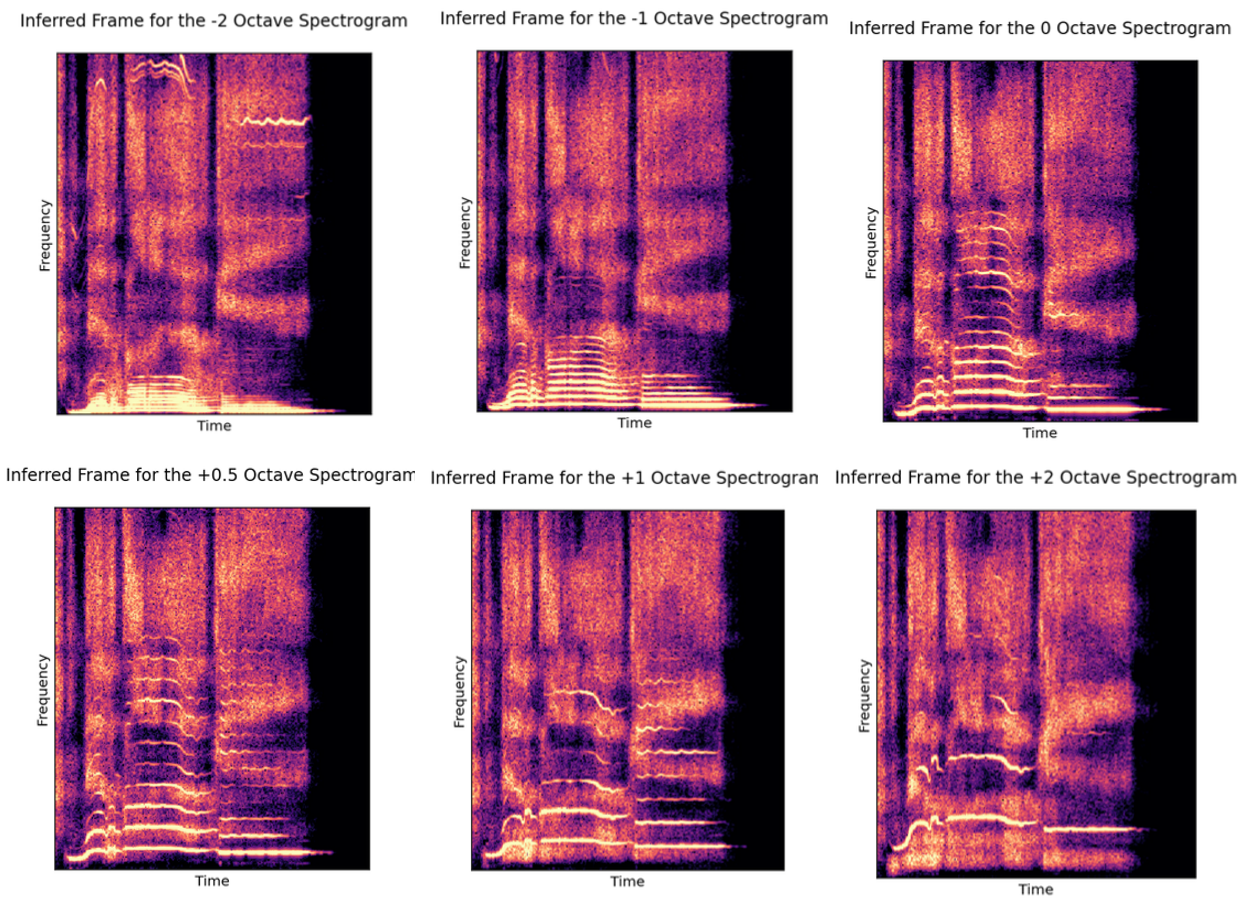
\includegraphics[width=\textwidth]{research/results/TaylorSwift/InferredTranspositions.png}
    \caption{(Taylor Swift) Inferred spectrogram frames at various octave transpositions realative to F0 at a certain timegrame in the original frame}
\end{figure}

\begin{figure}[H]
    \centering
    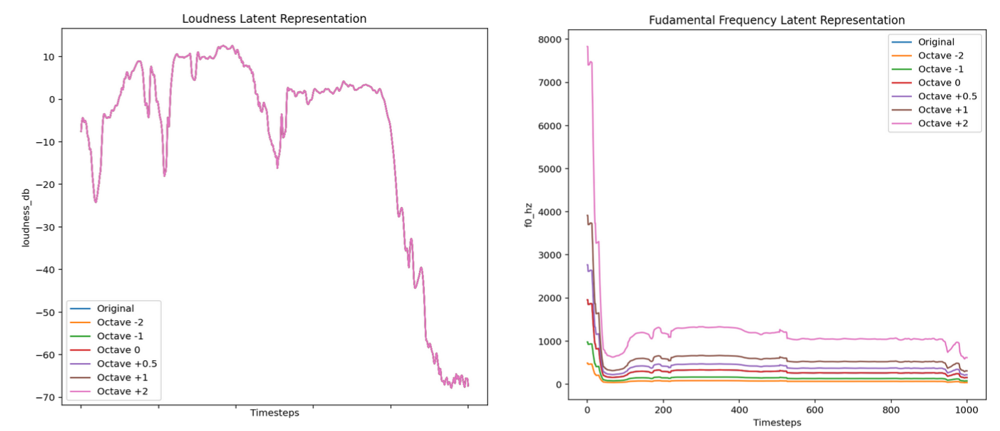
\includegraphics[width=\textwidth]{research/results/TaylorSwift/InferredTranspositionsGraphs.png}
    \caption{(Taylor Swift) Latent F0 and loudness features for various octave transpositions realative to F0 over timesteps throughout the frame}
\end{figure}

\begin{figure}[H]
    \centering
    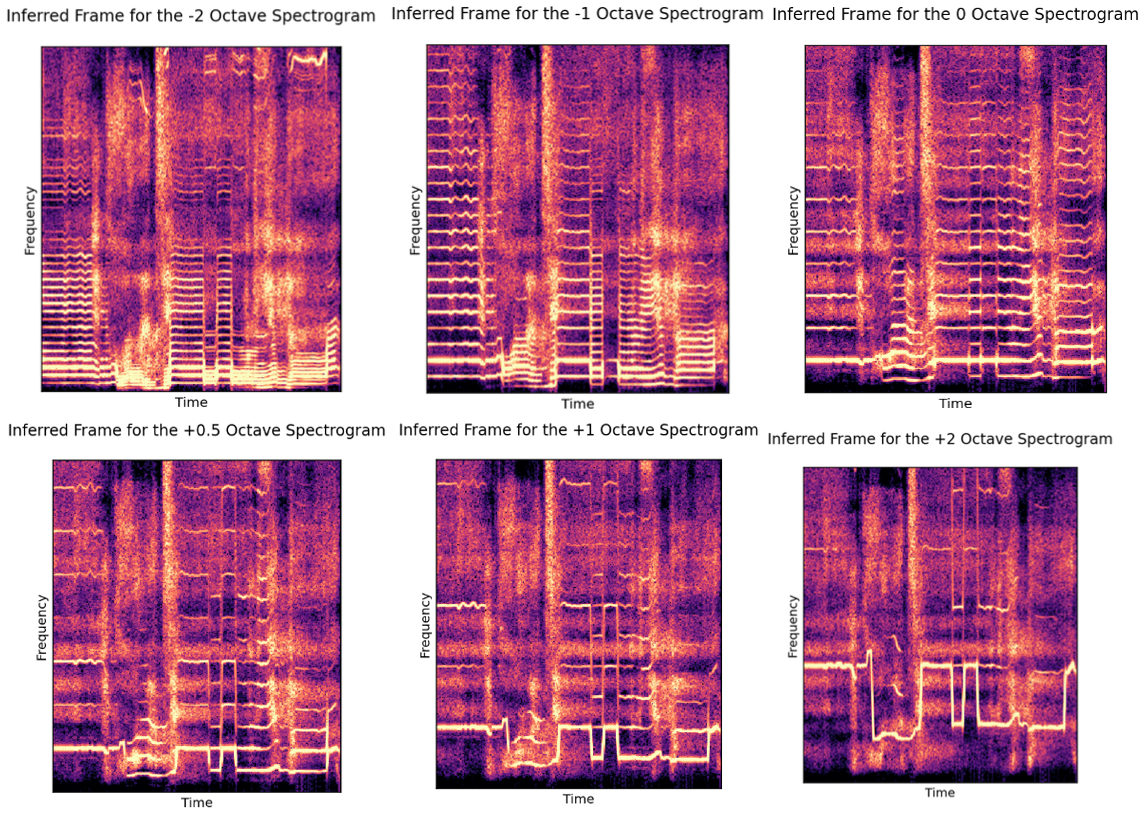
\includegraphics[width=\textwidth]{research/results/Coldplay/InferredTranspositions.png}
    \caption{(Coldplay) Inferred spectrogram frames at various octave transpositions realative to F0 at a certain timegrame in the original frame}
\end{figure}

\begin{figure}[H]
    \centering
    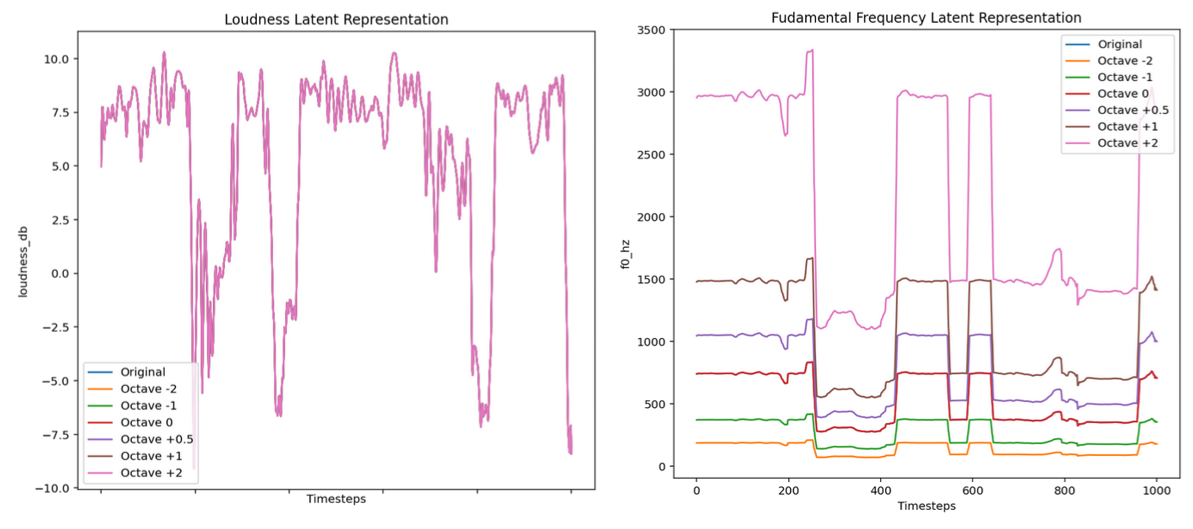
\includegraphics[width=\textwidth]{research/results/Coldplay/InferredTranspositionsGraphs.png}
    \caption{(Coldplay) Latent F0 and loudness features for various octave transpositions realative to F0 over timesteps throughout the frame}
\end{figure}

\subsection{Fixing F0}

The final pitch related test was fixing F0 to the mean value of F0 throughout the frame to see how the models would perform under unnatural pitch conditions.

Both models could fix the pitch to the mean value of F0 in the frame. This fixing is heard and can be seen visibly from the inferred spectrogram images where the harmonic components are at lines of constant frequency, unlike the original where they vary.

Additionally, words were still able to be synthesised and accurately heard, suggesting the model was able to learn the underlying phonemes of speech.

This result is excellent, mimicking what was founded in the speech DDSP research\cite{SpeechDDSP} (whose code was not publicly available). Further experiments were done with similar degrees of success in varying the pitch to other amounts, e.g. 100Hz and 500Hz. Again, however, the quality of results broke down at the extremes. The breakdown was evidenced by the harmonic again sounding more like a separate sound, with the whispers producing the actual words.

Sadly, timbral quality was reduced when F0 was fixed, with the output sounding more robotic and the original timbre being lost. Timbral loss is to be expected, however, as the original harmonic plus noise model was not designed with timbre transfer specifically in mind\cite{OriginalDDSP}.

\begin{figure}[H]
    \centering
    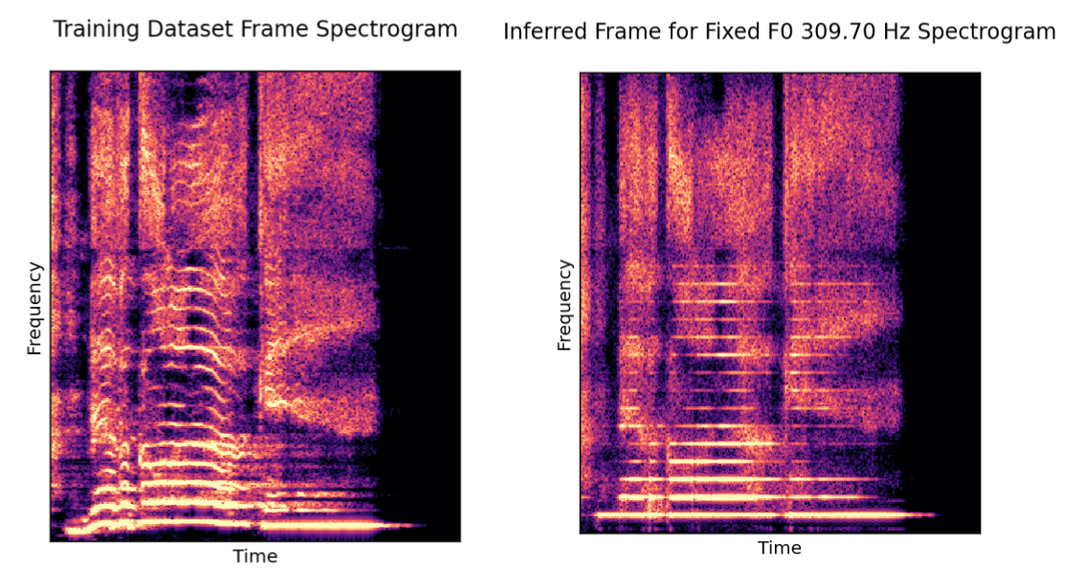
\includegraphics[width=\textwidth]{research/results/TaylorSwift/FixedF0.png}
    \caption{(Taylor Swift) Training dataset and fixed F0 spectrogram frames}
\end{figure}

\begin{figure}[H]
    \centering
    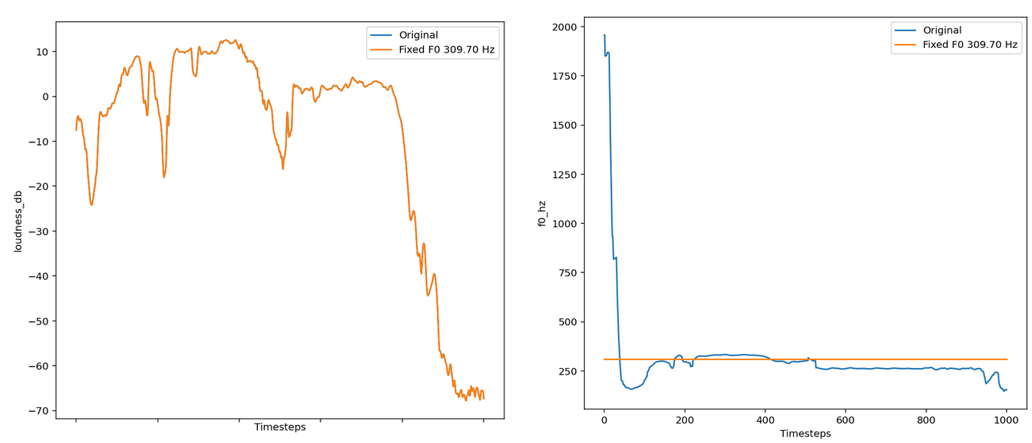
\includegraphics[width=\textwidth]{research/results/TaylorSwift/FixedF0Graphs.png}
    \caption{(Taylor Swift) Latent information on loudness and F0 over timesteps throughout the frame. The mean F0 was used to fix F0 throughout the frame}
\end{figure}

\begin{figure}[H]
    \centering
    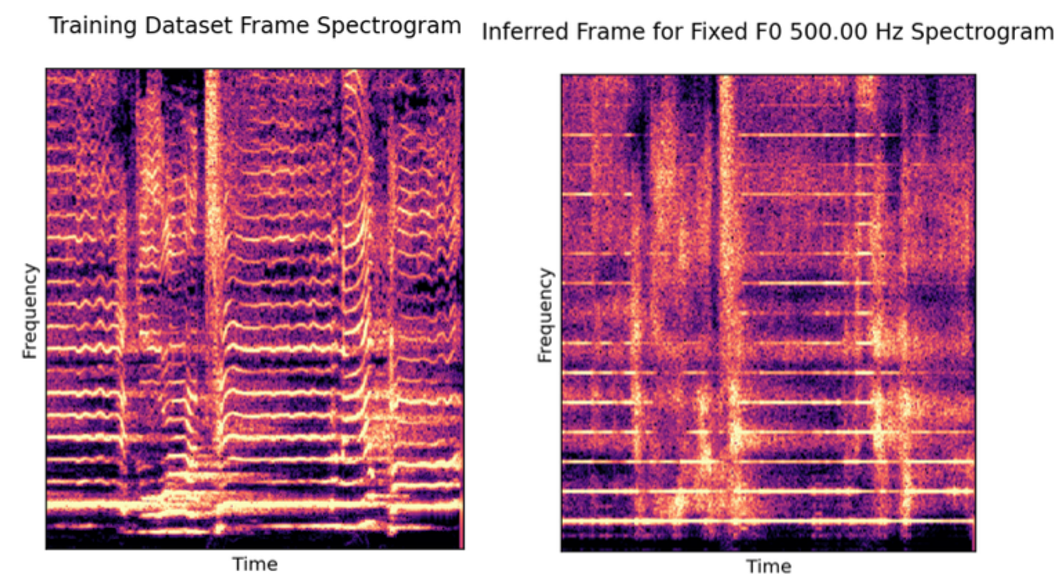
\includegraphics[width=\textwidth]{research/results/Coldplay/FixedF0.png}
    \caption{(Coldplay) Training dataset and fixed F0 spectrogram frames}
\end{figure}

\begin{figure}[H]
    \centering
    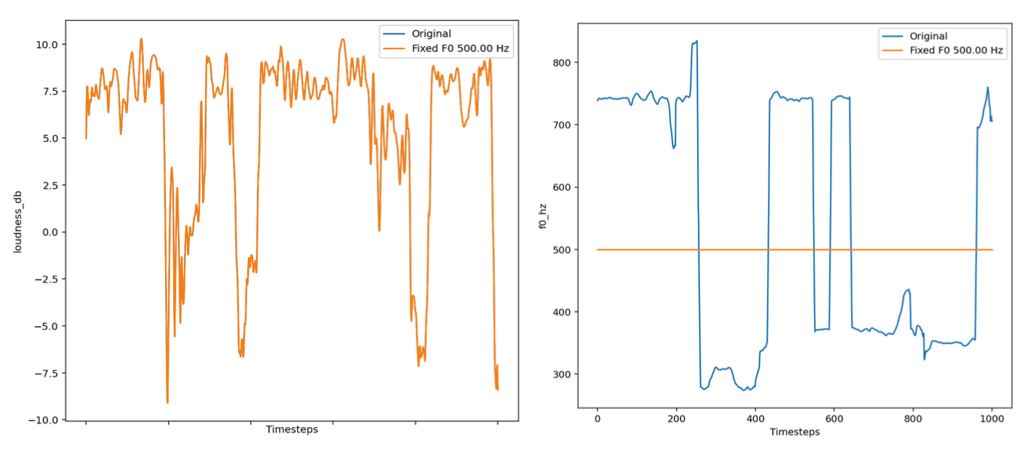
\includegraphics[width=\textwidth]{research/results/Coldplay/FixedF0Graphs.png}
    \caption{(Coldplay) Latent information on loudness and F0 over timesteps throughout the frame. The mean F0 was used to fix F0 throughout the frame}
\end{figure}

\subsection{Modifying Loudness}

Unfortunately, modification of the loudness latent vector did not alter the loudness of any inferred frames, and this could be caused by, perhaps, the decoder learning to ignore the latent loudness vector.

Alternatively, there may be some architectural issues with the modified decoder. For example, the DDSP library's authors significantly redesigned the loudness and power calculations with the version 3 release. Unfortunately, the Singing DDSP decoder used the older version 1. The discovery of any technical problems is beyond the scope of this thesis.

\subsection{Timbral Transfer}

The Taylor Swift model was selected for the timbral transfer tasks due to its better performance in the pitch transfer tests. For both male and female voice tests, vocals were successfully synthesised, and it was clear what words were being pronounced. Pitch was also accurately modelled for both cases. Success outside of the training set suggests that the model had successfully been generalised and had learned the underlying phonemes of human speech from spectrograms.

For the timbral transfer, the following songs were used:

\vspace{0.5cm}
\framebox[1.1\width]{
    \begin{minipage}{0.8\textwidth}
        \begin{itemize}
            \item \textbf{(Male Voice) Lewis Capaldi - \textit{Someone You Loved}}
            \item \textbf{(Female Voice) Birdy - \textit{Deep End}}
        \end{itemize}
    \end{minipage}
}
\vspace{0.5cm}

Sadly, the timbral transfer did not occur, with each inferred frame sounding similar to the source artist and not that of the training dataset. This result suggests that the model had learned to transfer timbre from the original vocal frame to the synthesised frame. Timbral quality was also reduced, sounding more unnatural, suggesting that perfect generalisation was not fully achieved. 

\begin{figure}[H]
    \centering
    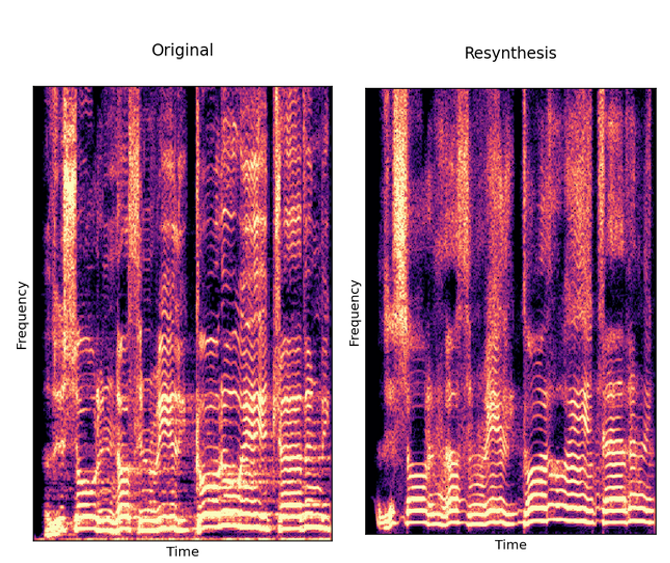
\includegraphics[width=\textwidth]{research/results/LewisCapaldi/TimbralTransfer.png}
    \caption{Lewis Capaldi timbral transfer test showing a comparison between the orignal and infererd spectrogram frames using the Taylor Swift model}
\end{figure}

\begin{figure}[H]
    \centering
    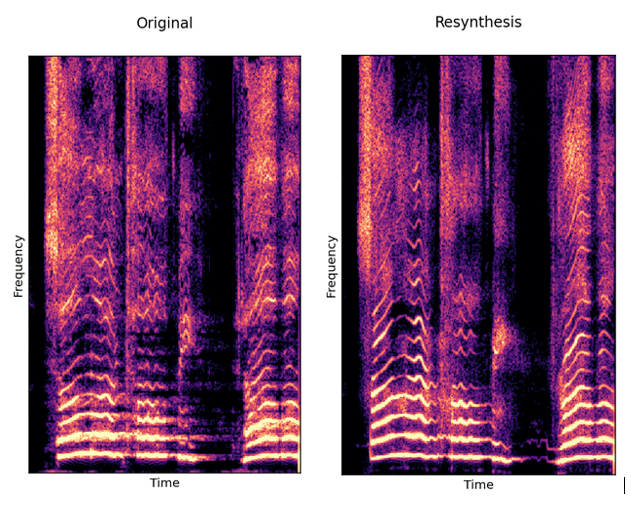
\includegraphics[width=\textwidth]{research/results/Birdy/TimbralTransfer.png}
    \caption{Birdy timbral transfer test showing a comparison between the oriignal and infererd spectrogram frames using the Taylor Swift model}
\end{figure}

\subsection{Inference with Instrumentals}

The Taylor Swift model was then used to infer a frame featuring the instrumental and vocal version of the song Deep End (i.e. the original song before passing through the Spleeter model).

The DDSP model managed to extract vocals from the track with instrumentals. Even more significant, there was no leakage of instrumentals in the inferred frame, suggesting that the model had isolated features unique to the human voice instead of more general noise features.

This result shows that the DDSP model is very flexible, being able to carry out source separation tasks similar to the Spleeter library\cite{Spleeter}; this was not demonstrated in the previous DDSP papers.

The inferred frames from the tracks with and without instrumentals sounded similar; however, F0 estimation in the frame with instrumentals could be better. Inaccurate F0 estimation is likely a limitation of using CREPE pitch estimation on a track with multiple parts simultaneously.

\begin{figure}[H]
    \centering
    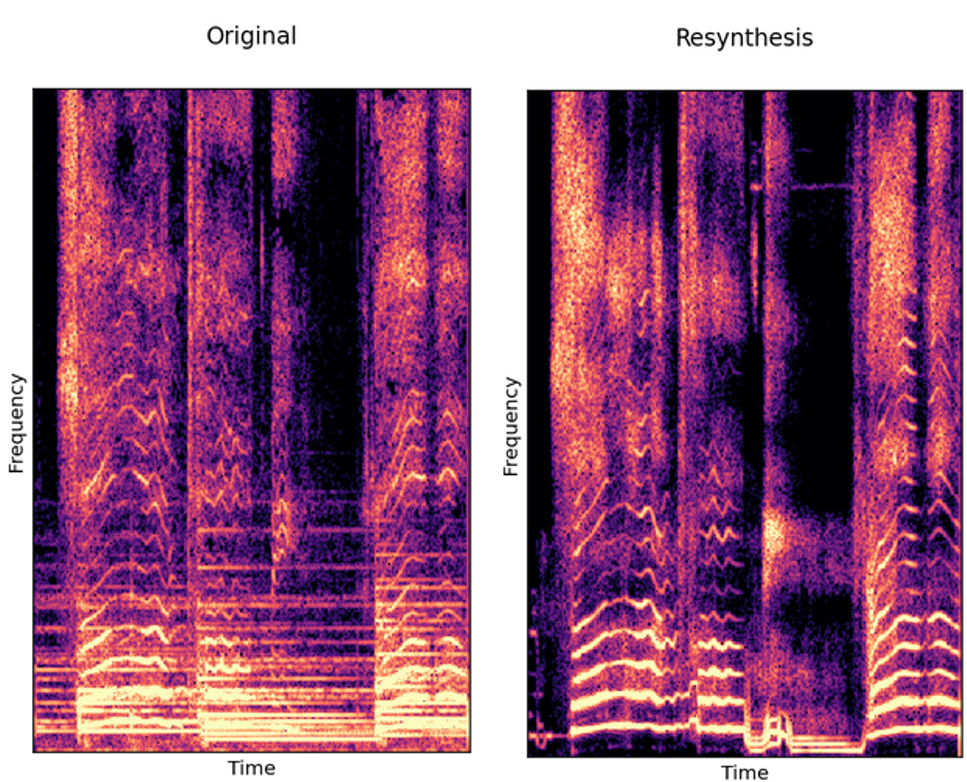
\includegraphics[width=\textwidth]{research/results/Birdy/InferenceWithInstrumentals.png}
    \caption{Birdy instrumental and vocals inference test using the Taylor Swift model, showing the original and infered spectrogram frames}
\end{figure}

\subsection{General Problems}

Along with the loudness perception problem, others were encountered during all inferencing tests:

\begin{enumerate}
    \item At low loudness levels, the CREPE model could not accurately detect the pitch of the audio sample. This lack of accuracy caused the fundamental frequency to jump around, sometimes appearing to jump up or down an octave, making the output sound jarring; this is evidenced in the Coldplay frames that all experience this problem. The DDSP authors suggested a potential solution was muting sections of the track where CREPE had low confidence in its prediction. Sadly, this fix could not work here due to the problems discussed around the loudness latent.
    \item The models failed to learn specific timbre related to the trained artist; this was especially apparent during the constant F0 test when the output sounded almost robotic. Lack of timbre transfer was foreseen as the DDSP architecture was not directly designed for timbre transfer.
    \item Similarly, when transferring timbre from another artist, the inferred sample sounded like the voice of the other artist more than it did that of the training dataset artist. However, this result could be attributed to the model's generalisation to synthesise the specific timbres derived from the noise characteristics of a test frame.
\end{enumerate}

The failure to learn timbre, as demonstrated throughout all the tests, could be the price paid for the ability of the model to understand, interpret, and synthesise any given voice.